\documentclass[12pt]{article}

\usepackage{sbc-template}

\usepackage{graphicx,url}

%\usepackage[brazil]{babel}   
\usepackage[utf8]{inputenc} 

\sloppy

\title{Inserção de metadados referentes a detecção de padrões no H.264}

\author{Tiago César Katcipis\inst{1}}


\address{Departamento de Informática e Estatística - Universidade Federal de Santa Catarina (UFSC)\\
  Santa Catarina -- SC -- Brazil
  \email{katcipis@inf.ufsc.br}
}

\begin{document} 

\maketitle

\begin{abstract}
To store and transmit video the use of encoders has been increasing, MPEG 4 part 10, also known as H.264, stands out among these encoders. This work integrates the Haar classifier to the reference MPEG 4 part 10 encoder to detect objects and explores the motion estimation algorithm of the encoder to track the detected objects. Detected objects and tracking information are represented in the form of metadata and bitstream are transported in the video messages using Supplemental Enhancement Information. The tests showed that the generated video is in accordance with the MPEG 4 part 10, together with a satisfactory computational performance. The results obtained in the decoder, retrieving the metadata and presenting them, were also satisfactory, showing the viability of building a object tracking system embedded on the encoder.
\end{abstract}
  
\begin{resumo} 
Para realizar o armazenamento e transmissão de vídeo tem se utilizado cada vez mais codificadores, dentre esses codificadores se destaca o MPEG 4 parte 10, também conhecido como H.264. Este trabalho integra um classificador Haar ao codificador de referência do padrão MPEG 4 parte 10 para realizar a detecção de objetos e explora o algoritmo de estimativa de movimento do codificador para realizar o tracking do objeto. Os objetos detectados e as informações de tracking são representados na forma de metadados e são transportados no bitstream do vídeo utilizando mensagens Supplemental Enhancement Information. Os testes realizados mostram que o codificador gerou vídeos em conformidade com o padrão  MPEG 4 parte 10, junto com um desempenho computacional satisfatório. Os resultados obtidos no decodificador, ao recuperar os metadados e apresentá-los, também foram satisfatórios mostrando a viabilidade de construir um sistema de tracking de objetos embutido no codificador.
\end{resumo}

\section*{Introdução}

Atualmente tem se tornado comum em soluções de segurança o uso de detecção de padrões como detecção facial, detecção de objetos específicos, cercas virtuais, alarmes, etc. Dispositivos de gravação de vídeo em alta definição estão se tornando cada vez mais acessíveis, estando presentes até mesmo em celulares, porém como é inviável dispor de longos trechos de vídeo em alta resolução sem compactação pois estes consomem um grande espaço de armazenamento e não é possível transmiti-los em larga escala com os meios de comunicação existentes, esses vídeos em alta definição são usualmente compactados.

A maior parte dos algoritmos de identificação de objetos e algoritmos biométricos trabalham com informações não codificadas, nesse caso, o processamento de multiplos vídeos exigiria que esses vídeos fossem decodificados primeiro e então processados. Alguns algoritmos de identificação de objetos trabalham com informações codificadas, um exemplo é o detector de faces proposto em \cite{faceDetectionH264}, mas na conclusão do mesmo é possível se observar que apesar do resultado ser satisfatório, o processamento em um identificador de objetos utilizando informações brutas foi superior (no caso a comparação foi realizada com o classificador Haar do OpenCV).

Considerando que a busca por objetos de interesse fosse realizada no vídeo compactado (não sendo necessário decodificar o vídeo), em um caso de uso como o de um aeroporto onde existem muitas câmeras de segurança, ainda seria necessário um grande poder computacional para realizar a busca de objetos de interesse em todos vídeos ao mesmo tempo, já que normalmente se espera que um sistema de segurança tenha um tempo de resposta rápido. 

Dessa maneira é interessante obter a maior quantidade possível de metadados a respeito de objetos de interesse, na fonte do vídeo, de maneira integrada ao processo de codificação, reaproveitando ao máximo qualquer informação que o processo de codificação possa fornecer. Ao invés de analisar os vídeos, será realizada uma análise dos metadados. Se um vídeo muito longo não possui nenhum metadado, não será necessário analisá-lo. Como metadados pode-se citar a presença de um objeto de interesse (sua posição e tamanho), padrões de movimento (útil em cercas virtuais) ou o objeto de interesse em alta resolução não compactado (facilita o processamento posterior desse objeto em um algoritmo biométrico).

Ao utilizar ao máximo as informações que o próprio codificador gera para realizar a identificação de padrões é interessante transportar os metadados gerados dentro do próprio bitstream do vídeo, isso facilita o desenvolvimento de um chip codificador na solução, pois não é necessário que os metadados encontrados sejam enviados a aplicação para serem transportados de outra maneira. Neste artigo será apresentado um estudo da integração de um algoritmo de detecção de padrões com as informações de estimativa de movimento calculadas pelo codificador MPEG 4 parte 10, gerando um \textit{tracker} de objetos, capaz de enviar também objetos de interesse não compactados.

A estrutura deste artigo apresenta-se da seguinte forma. A seção \ref{art:extract} explica como os metadados são extraídos e representados no sistema. A seção \ref{art:codificador} apresenta as alterações realizadas no codificador, utilizando os componentes explicados em \ref{art:extract}. Na seção \ref{art:testes} serão apresentados os testes realizados com o sistema desenvolvido. A seção \ref{art:conclusao} conclui este artigo, apresentando as contribuições deste trabalho e os trabalhos futuros.


\section*{Extração e representação dos metadados}
\label{art:extract}

\subsection{ Módulo extracted\_metadata }

A classe \textit{Extracted\_Metadata} abstrai a serialização, desserialização, salvamento e destruição dos diferentes tipos de metadados. O método \textit{serialize} é responsável pela serialização, uma vez serializado o metadado será inserido diretamente no \textit{bitstream} do vídeo como uma mensagem SEI (\textit{Supplemental Enhancement Information}). 

Foram implementadas duas subclasses da classe \textit{Extracted\_Metadata}, para representar os metadados extraídos:

\begin{itemize}

        \item \textit{ Extracted\_Y\_Image }: Representa o plano luma de um objeto de interesse, é composto basicamente do plano luma com o seu comprimento e altura. Ao detectar um objeto de interesse é possível extrair apenas o objeto e inserí-lo no bitstream. O objeto pode ser recuperado no decoder e salvo em um arquivo.
        \item \textit{ Extracted\_Object\_Bounding\_Box }: Representa uma caixa delimitadora envolta de um objeto de interesse. Ela é composta de um identificador único do objeto, as coordenadas (x, y) da caixa, sua altura e seu comprimento. Com as informações de coordenadas da caixa delimitadora é possível desenhar a caixa delimitadora diretamente no vídeo e com o identificador único é possível realizar o \textit{tracking} do objeto ao longo do vídeo.

\end{itemize}


\subsection{ Módulo metadata\_extractor }

Este módulo é responsável pela extração de metadados a partir de quadros brutos e das informações de estimativa de movimento fornecidas. Extraindo metadados do tipo \textit{ExtractedObjectBoundingBox} e \textit{ExtractedYImage}. Para realizar a detecção de um objeto de interesse no quadro foi utilizado o classificador Haar do OpenCV. O termo histerese se refere a quantidade de quadros necessários para realizar a execução do classificador Haar, gerando um atraso configurável na detecção de um novo objeto, ou ao confirmar a existência de um objeto previamente detectado. O método \textit{extract\_object\_bounding\_box} extrai do quadro uma caixa delimitadora que representa a área onde se encontra o objeto de interesse no quadro e retorna como um objeto \textit{ExtractedMetadata}. 

As histereses configuradas, junto com as informações de estimativa de movimento, visam utilizar os algoritmos já existentes no codificador para reduzir o custo computacional do \textit{tracking} de um objeto no vídeo. Ao invés de realizar o processamento de todos os quadros brutos no classificador Haar para realizar o \textit{tracking} do objeto ao longo do vídeo, a histerese diminui o custo computacional por atualizar a posição do objeto em intervalos fixos. Os vetores de movimento calculados pelo codificador são utilizados para suavizar o \textit{tracking}, estimando a nova posição do objeto enquanto a histerese de \textit{tracking} não estoura.

\begin{figure}[H]
\centering
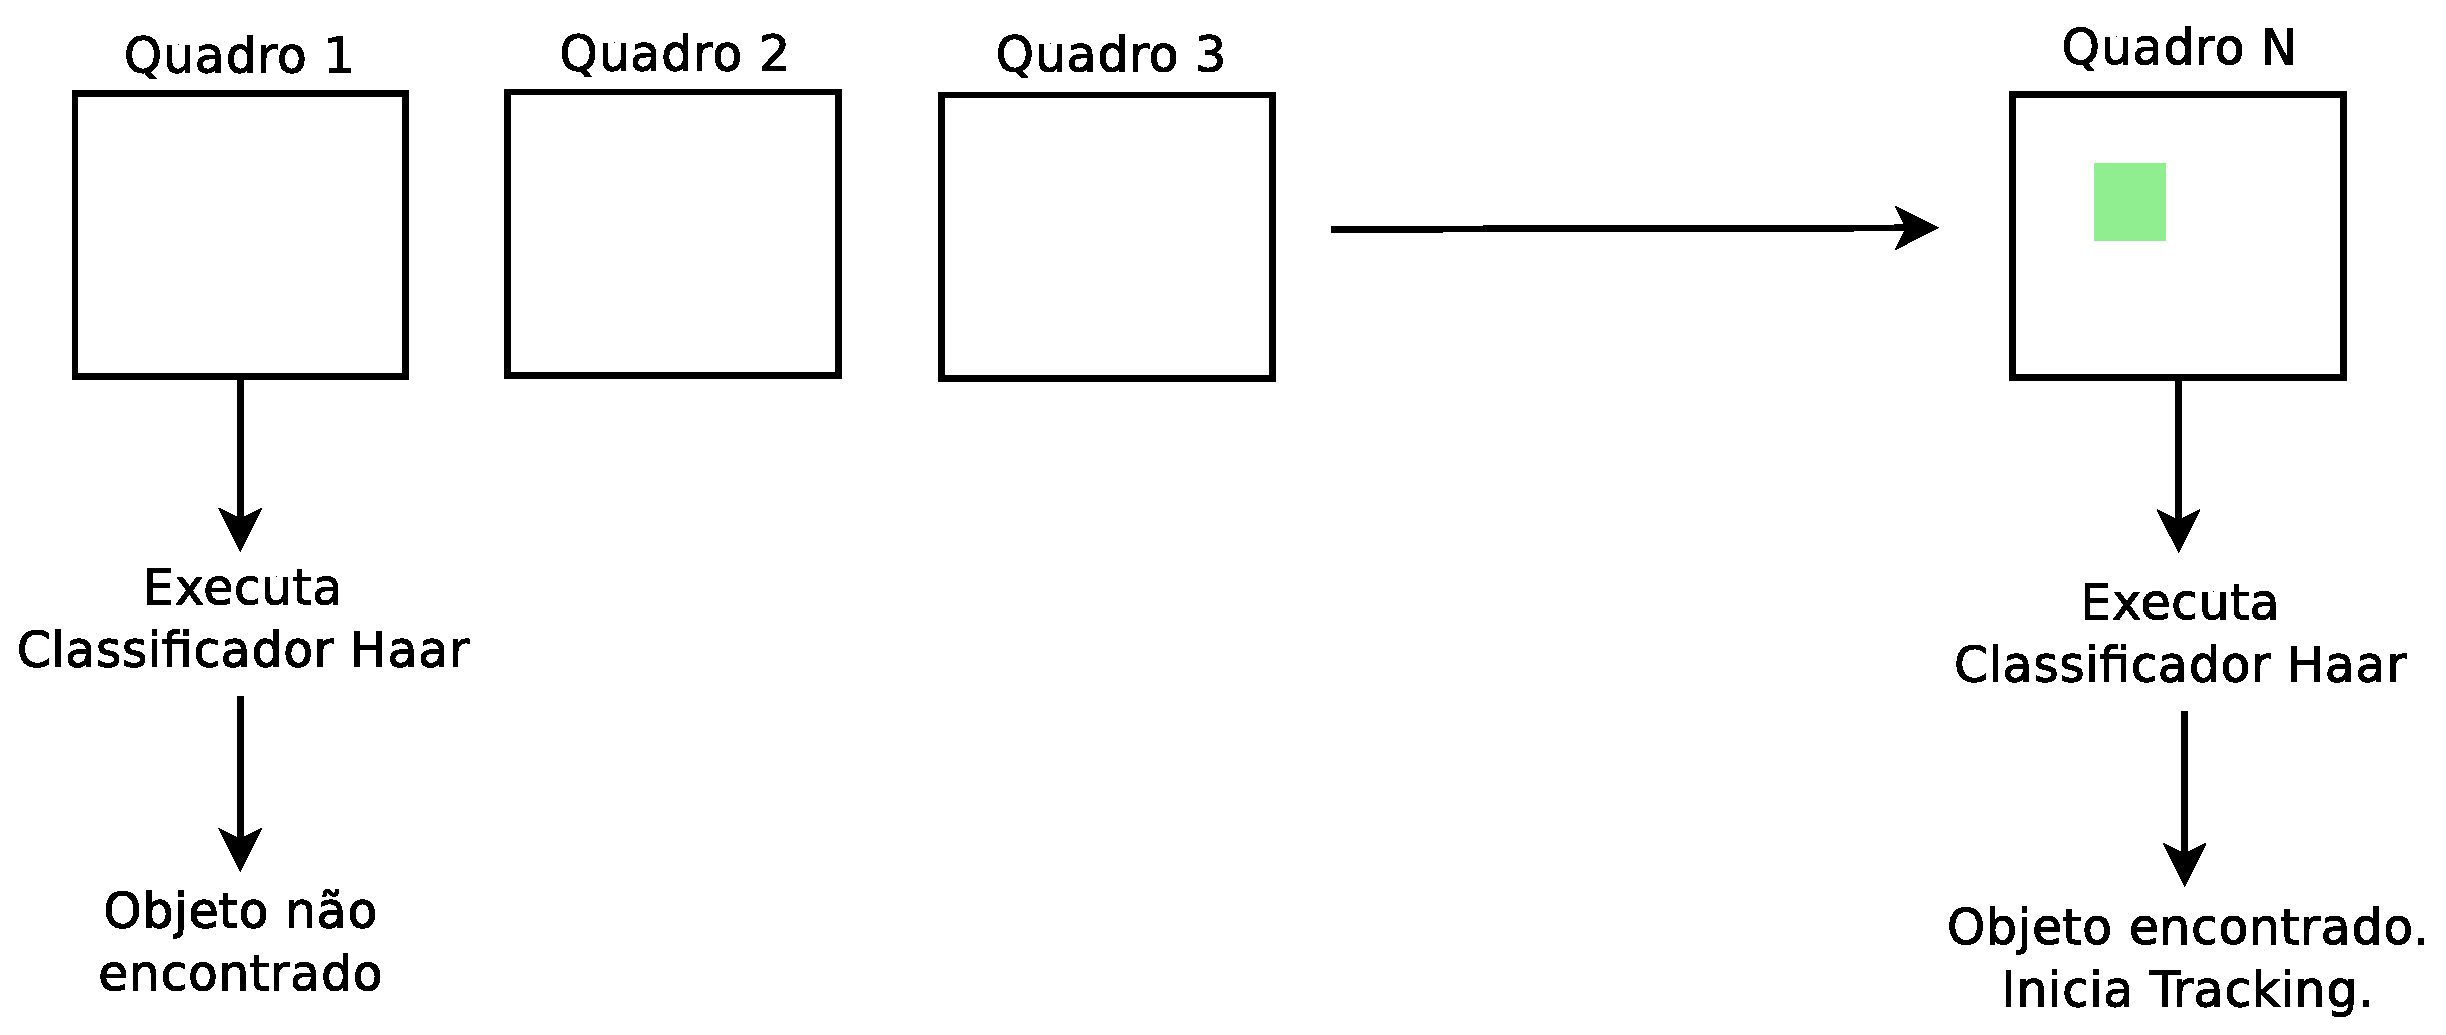
\includegraphics[scale=0.4]{../imagens/fig23.eps}
\caption{Exemplo do funcionamento da histerese de busca.}
\label{fig:search_histeresys_example_artigo}
\end{figure}

O mesmo se dá quando o objeto já foi detectado, não é necessário executar o classificador em todos os quadros, os vetores de estimativa de movimento nos dão uma idéia aproximada da posição do objeto, até que seja alcançada a histerese de \textit{tracking}.

\begin{figure}[H]
\centering
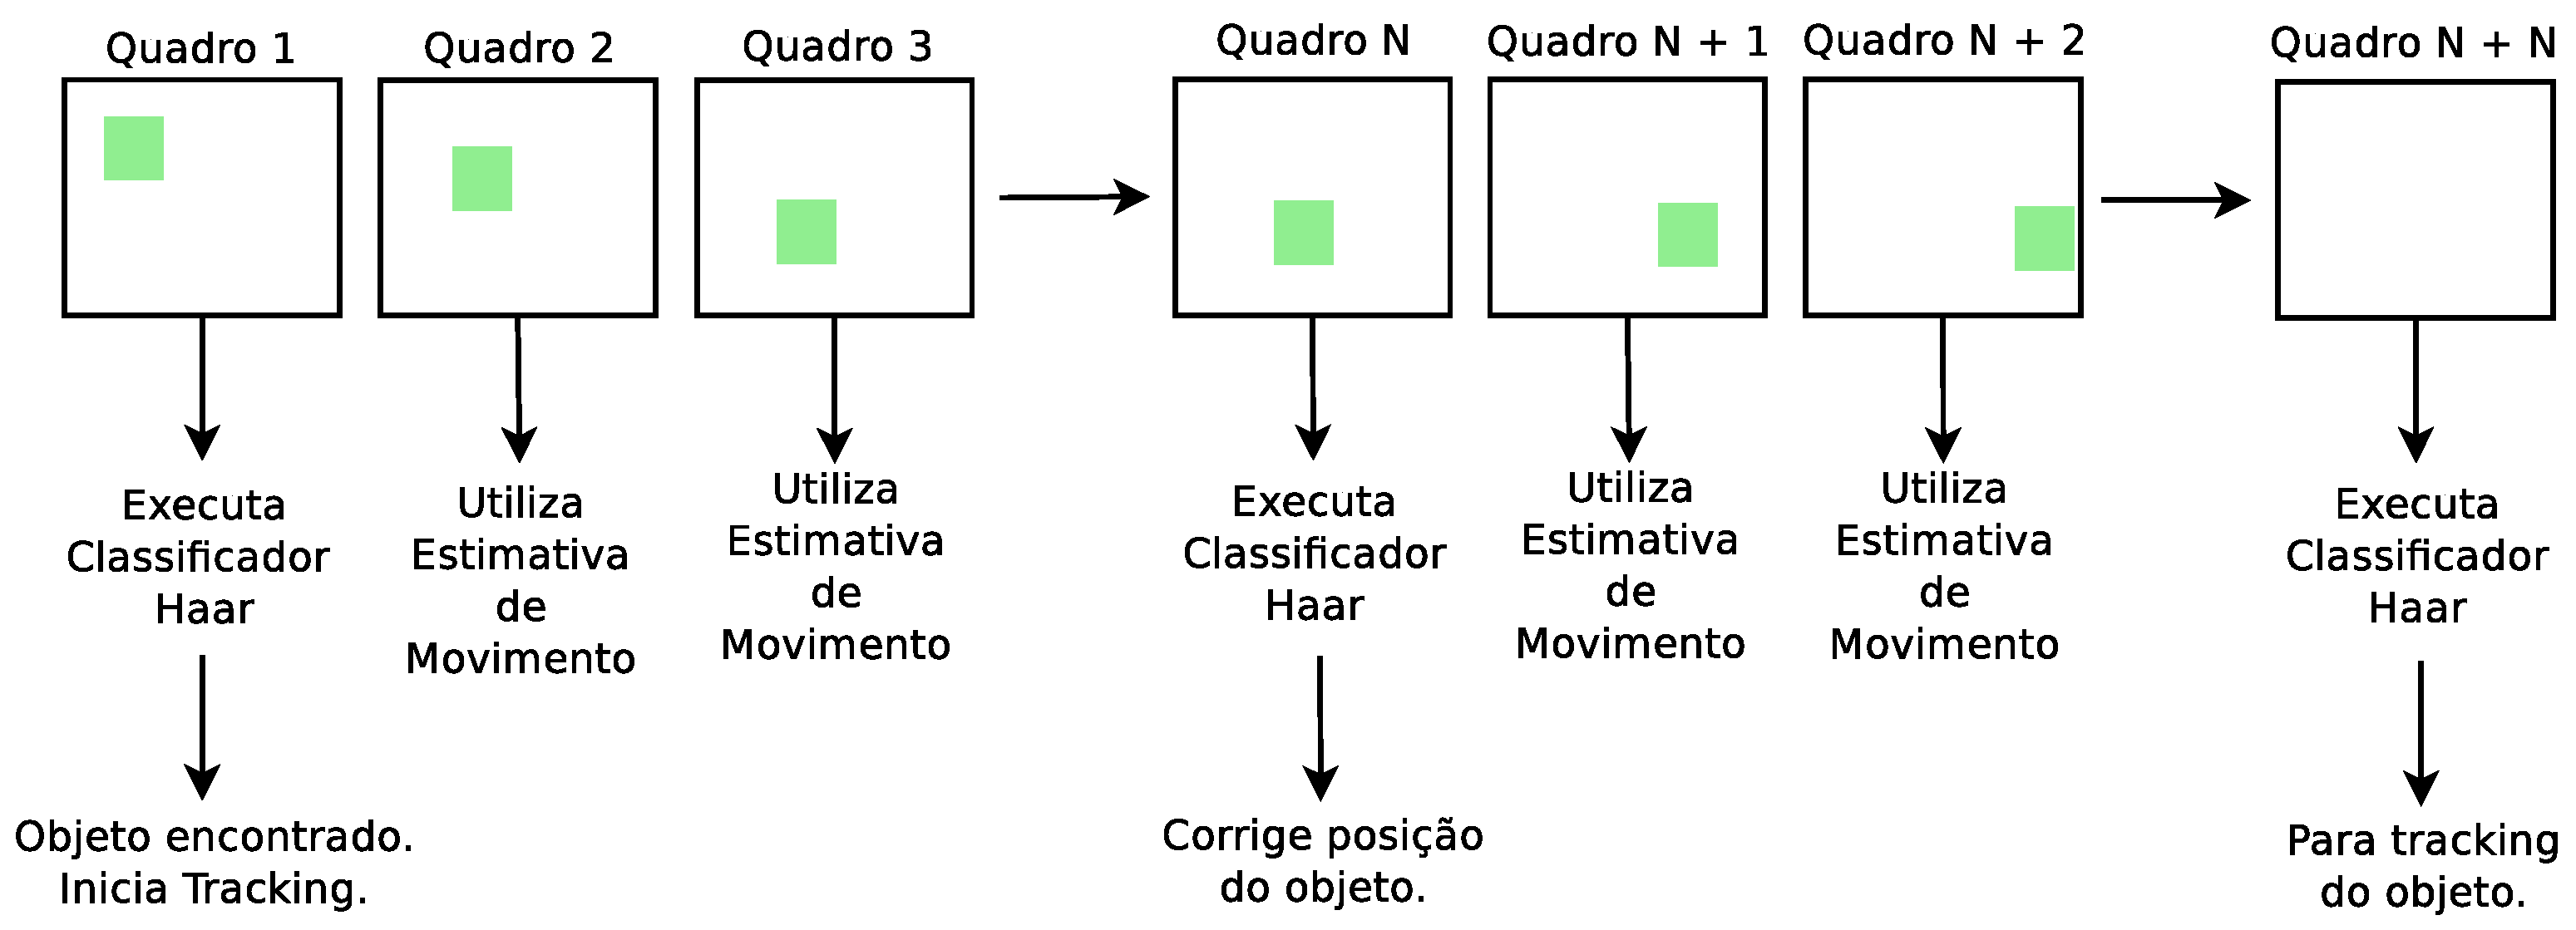
\includegraphics[scale=0.3]{../imagens/fig24.eps}
\caption{Exemplo do funcionamento da histerese de \textit{tracking}.}
\label{fig:tracking_histeresys_example_artigo}
\end{figure}


\section*{Alterações realizadas no codificador}
\label{art:codificador}

O codificador utilizado no desenvolvimento do sistema foi o que se encontra no software de referência desenvolvido pelo JVT (Joint Video Team) e hospedado pelo Instituto Fraunhofer para telecomunicações, Instituto Heinrich Hertz. Esta implementação foi utilizada por ela ser referência para pesquisas e verificação de conformidade com a norma, a versão utilizada foi a 17.2.

Dentro da função \textit{encode\_one\_frame}, o processamento do quadro bruto é realizado logo após a chamada de função \textit{process\_image}, neste momento também ocorre a extração do metadado e o mesmo é salvo no bitstream na forma de mensagem SEI \textit{Unregistered Userdata}. Além dos quadros brutos, outra informação importante para o extrator de metadados são os vetores de movimento dos blocos. Na função \textit{code\_a\_plane} antes da chamada de função \textit{DeblockFrame} todo o processo de estimativa de movimento já está completo, neste ponto é que os vetores de estimativa de movimento do quadro são repassados ao extrator de metadados para que ele realize a estimativa de movimento do objeto detectado (se o extrator estiver realizando \textit{tracking}).

\section*{Testes realizados}
\label{art:testes}

Todos os testes utilizaram o mesmo arquivo de treinamento \textit{haarcascade\_frontalface\_alt.xml}, que realiza a busca de faces frontais, este arquivo vem junto com a distribuição do OpenCV (que pode ser encontrada em http://sourceforge.net/projects/opencvlibrary/files) no diretório \textit{data/haarcascades}. O tamanho mínimo do objeto de interesse configurado em todos os testes foi de 30 x 30 pixels.

A configuração da máquina e o sistema operacional utilizados nos testes foi:


\begin{itemize}
        \item Processador Pentium(R) Dual-Core E5200 á 2.50GHz.
        \item 4 gigabytes de memória RAM.
        \item Sistema operacional Ubuntu 11.04 32 bits.
\end{itemize}

Foram realizados 5 testes em cada vídeo, todos com a mesma configuração de codificação:

\begin{itemize}
        \item Sem \textit{tracking} de objetos.

	\item Com \textit{tracking} ativado, com histerese de busca = 1 e histerese de \textit{tracking} = 1. Dessa maneira as informações de estimativa de movimento do codificador não são utilizadas, o \textit{tracking} é realizado utilizando apenas o classificador Haar.

	\item Com \textit{tracking} ativado, com histerese de busca = 5 e histerese de \textit{tracking} = 10. Essa configuração faz um menor uso das informações de estimativa de movimento para realizar \textit{tracking} de um objeto.

         \item Com \textit{tracking} ativado, com histerese de busca = 10 e histerese de \textit{tracking} = 30. Essa configuração depende mais das informações de estimativa de movimento para realizar \textit{tracking} de um objeto.

         \item Com \textit{tracking} ativado, com histerese de busca = 10 e histerese de \textit{tracking} = 60. Essa configuração é a que mais depende mais das informações de estimativa de movimento para realizar \textit{tracking} de um objeto.
\end{itemize}


\subsection{ Vídeo Foreman - CIF - 300 quadros }


Esse vídeo pode ser encontrado em http://media.xiph.org/video/derf/y4m/foreman\_cif.y4m e possui 3 situações diferentes, uma face frontal, a face fica de perfil em alguns momentos, e depois a face sai do vídeo.

Especificações do vídeo:

\begin{itemize}
        \item quadros por segundo = 29.97.
        \item total de quadros    = 300.
        \item comprimento         = 352 pixels.
        \item altura              = 288 pixels.
        \item espaço de cor       = YUV, 4:2:0.
\end{itemize}


\begin{table}[H]
\begin{center}
\begin{tabular}{|p{2.3cm}|p{2.3cm}|p{2.3cm}|p{2.3cm}|p{2.3cm}|p{2.3cm}|}
\hline
\textbf{} & \textbf{\textit{Tracking} Desabilitado} & \textbf{\textit{Tracking} habilitado, sem histerese} & \textbf{Histerese de busca = 5, \textit{tracking} = 10} & \textbf{Histerese de busca = 10, \textit{tracking} = 30} & \textbf{Histerese de busca = 10, \textit{tracking} = 60} \\
\hline
Atraso no tempo total codificação & 0\% & 9,87\% & 1,75\% & 0,85\% & 0,65\% \\
\hline
Aumento bitstream  & 0\% & 0,36\% & 0,43\% & 0,55\% & 0,66\% \\
\hline
\end{tabular}
\caption{Desempenho do sistema com o vídeo Foreman.}
\label{tab:space_overhead}
\end{center}
\end{table}

Com a detecção de objetos ocorrendo em todos os quadros percebe-se uma alta taxa de falsos negativos, já que o rosto no vídeo fica de perfil em alguns momentos e o classificador Haar não consegue identificar o rosto em perfil, perdendo assim o \textit{tracking} do rosto. Com a detecção de objetos em todos os quadros também ocorreu um falso positivo quando a camêra se move e deixa de gravar o rosto. A medida que a histerese de \textit{tracking} é aumentada, além de não ocorrer o falso positivo, os movimentos que o rosto realiza são acompanhados com maior suavidade e com uma menor taxa de falsos negativo (com a histerese de \textit{tracking} configurada para 60 quadros não ocorreu nenhum falso negativo). 


\subsection{ Vídeo Akiyo - QCIF - 300 quadros }


Esse vídeo pode ser encontrado em http://media.xiph.org/video/derf/y4m/akiyo\_qcif.y4m e consiste basicamente de 300 quadros positivos (existe o objeto de interesse ao longo de todo o vídeo, nesse caso uma face frontal).


Especificações do vídeo:

\begin{itemize}
        \item quadros por segundo = 29.97.
        \item total de quadros    = 300.
        \item comprimento         = 176 pixels.
        \item altura              = 144 pixels.
        \item espaço de cor       = YUV, 4:2:0.
\end{itemize}


\begin{table}[H]
\begin{center}
\begin{tabular}{|p{2.3cm}|p{2.3cm}|p{2.3cm}|p{2.3cm}|p{2.3cm}|p{2.3cm}|}
\hline
\textbf{} & \textbf{\textit{Tracking} Desabilitado} & \textbf{\textit{Tracking} habilitado, sem histerese} & \textbf{Histerese de busca = 5, \textit{tracking} = 10} & \textbf{Histerese de busca = 10, \textit{tracking} = 30} & \textbf{Histerese de busca = 10, \textit{tracking} = 60} \\
\hline
Atraso no tempo total codificação & 0\% & 10,94\% & 1,27\% & 0,59\% & 0,39\% \\
\hline
Aumento bitstream  & 0\% & 3,83\% & 3,77\% & 3,71\% & 3,71\% \\
\hline
\end{tabular}
\caption{Desempenho do sistema com o vídeo Akiyo.}
\label{tab:space_overhead}
\end{center}
\end{table}

Como este vídeo é composto de apenas uma pessoa, realizando pequenos movimentos suaves, os resultados com histerese de \textit{tracking} alta foram bons. A ativação de detecção de objetos em todos os quadros, utilizando apenas o classificador Haar para realizar o \textit{tracking}, tornou o processo de codificação aproximadamente 10,94\% mais lento. 


\subsection{ Vídeo \textit{Pedestrian area} - 375 quadros - 1080p (1920 x 1080) }

Esse vídeo pode ser encontrado em http://media.xiph.org/video/derf/y4m/pedestrian\_area\_1080p25.y4m. Ele consiste basicamente de vários pedestres caminhando em uma rua, possui faces frontais e faces em perfil se movendo continuamente. 

Especificações do vídeo:

\begin{itemize}
        \item quadros por segundo = 25.
        \item total de quadros    = 375.
        \item comprimento         = 1920 pixels.
        \item altura              = 1080 pixels.
        \item espaço de cor       = YUV, 4:2:0.
\end{itemize}


\begin{table}[H]
\begin{center}
\begin{tabular}{|p{2.3cm}|p{2.3cm}|p{2.3cm}|p{2.3cm}|p{2.3cm}|p{2.3cm}|}
\hline
\textbf{} & \textbf{\textit{Tracking} Desabilitado} & \textbf{\textit{Tracking} habilitado, sem histerese} & \textbf{Histerese de busca = 5, \textit{tracking} = 10} & \textbf{Histerese de busca = 10, \textit{tracking} = 30} & \textbf{Histerese de busca = 10, \textit{tracking} = 60} \\
\hline
Atraso no tempo total codificação & 0\% & 5,27\% & 0,08\% & 0,04\% & 0,005\% \\
\hline
Aumento bitstream  & 0\% & 0,207\% & 0,209\% & 0,211\% & 0,210\% \\
\hline
\end{tabular}
\caption{Desempenho do sistema com o vídeo \textit{Pedestrian area}.}
\label{tab:space_overhead}
\end{center}
\end{table}

Com a detecção de objetos ocorrendo em todos os quadros ocorre uma grande quantidade de falsos positivos, e a limitação de realizar o \textit{tracking} de apenas um objeto por vez ficou bem evidente já que neste vídeo existem diversas pessoas andando ao mesmo tempo o sistema consegue realizar o \textit{tracking} de algumas faces por um curto periodo de tempo, mas logo depois detecta outra face e passa a realizar o \textit{tracking} dessa face ao invés da que foi previamente detectada. 

A utilização das histereses alterou um pouco o comportamento do sistema (em geral ele manteve uma alta taxa de falsos positivos), a primeira detecção que ocorre com sucesso realiza o \textit{tracking} da face corretamente, mas após essa primeira detecção ocorre uma série de falsos positivos, e em algumas detecções positivas o \textit{tracking} não consegue acompanhar a face por ela estar se movendo rápido demais.


\subsection{ Vídeo \textit{Pedestrian area} - 375 quadros - 720p (1280 x 720) }


Neste teste a resolução do vídeo \textit{Pedestrian area} foi reduzida de \textit{1080p} (1920 x 1080) para \textit{720p} (1280 x 720), visando a constatação da diferença do impacto do sistema de \textit{tracking} ao processar o mesmo vídeo com resoluções diferentes. O escalonamento do vídeo foi realizado utilizando o Gstreamer.


\begin{table}[H]
\begin{center}
\begin{tabular}{|p{2.3cm}|p{2.3cm}|p{2.3cm}|p{2.3cm}|p{2.3cm}|p{2.3cm}|}
\hline
\textbf{} & \textbf{\textit{Tracking} Desabilitado} & \textbf{\textit{Tracking} habilitado, sem histerese} & \textbf{Histerese de busca = 5, \textit{tracking} = 10} & \textbf{Histerese de busca = 10, \textit{tracking} = 30} & \textbf{Histerese de busca = 10, \textit{tracking} = 60} \\
\hline
Atraso no tempo total codificação & 0\% & 11,09\% & 0,84\% & 0,44\% & 0,23\% \\
\hline
Aumento bitstream  & 0\% & 0,34\% & 0,37\% & 0,34\% & 0,35\% \\
\hline
\end{tabular}
\caption{Desempenho do sistema com o vídeo \textit{Pedestrian area - 720p}.}
\label{tab:space_overhead}
\end{center}
\end{table}

A diminuição da resolução do vídeo não gerou nenhuma diferença na qualidade do \textit{tracking}, porém foi possível perceber um aumento no atraso no tempo total de codificação em todas as configurações. 

\section*{Conclusão}
\label{art:conclusao}

Testes realizados tanto com o decodificador de referência como com o Gstreamer mostraram que o uso de mensagens \textit{Supplemental Enhancement Information} do tipo \textit{Unregistered Userdata} para transportar os metadados diretamente no \textit{bitstream} do vídeo não alteraram a conformidade do mesmo com o padrão, sendo possível exibir um vídeo com metadados embutidos em qualquer decodificador MPEG 4 parte 10. Executar o classificador Haar em todos os quadros do vídeo mostrou um aumento considerável no custo computacional do codificador. 

Utilizou-se informações de estimativa de movimento calculadas pelo codificador para estimar o movimento do objeto, evitando a necessidade de executar o classificador Haar em todos os quadros do vídeo, dessa maneira constatou-se uma significativa redução do custo computacional reutilizando informações geradas pelo processo de codificação. 

Como toda a extração do metadado e inserção dele dentro do \textit{bitstream} é feita internamente no codificador isso facilita a construção de um chip codificador H.264 que realize \textit{tracking} de objetos, esse chip codificador poderia ter grande parte do classificador Haar acelerado também em hardware, dentro do chip. Como pode ser visto em \cite{haarFPGA}, obtêm-se um grande aumento no desempenho da detecção de objetos ao utilizar o classificador implementado em uma FPGA. 

Este artigo mostrou a viabilidade de se utilizar a estimativa de movimento gerada pelo codificador para auxiliar o \textit{tracking} de objetos e do envio dessas informações através do \textit{bitstream} do vídeo. Além das informações de \textit{tracking} foi possível enviar o objeto detectado não compactado como metadado, o que pode ser útil em algoritmos de identificação biométrica. No momento da análise dos vídeos é necessário analisar apenas os metadados que estão inseridos no \textit{bitstream}, grande parte do processamento já foi realizado durante o processo de codificação.

Como possíveis trabalhos futuros, cita-se: 

\begin{itemize}
        \item Fazer um melhor uso das informações geradas pelo processo de codificação para gerar heurísticas mais inteligentes. Um exemplo seria utilizar histereses dinâmicas, quando existe muito movimento no vídeo as histereses diminuem, mas quando não existe movimento as histereses aumentam.
        \item Estender o sistema para realizar a detecção e \textit{tracking} de múltiplos objetos (com mesma forma) simultaneamente.
        \item Buscar no classificador Haar cálculos que já possam ter sido feitos pelo codificador, melhorando a integração dos dois.
        \item Utilizar outro algoritmo de detecção de padrões que tenha uma maior interseção com os algoritmos presentes no codificador.
        \item Utilizar apenas as informações de estimativa de movimento para a construção de cercas virtuais ou alarmes que não se importem com a forma do objeto mas com padrões de movimento suspeitos.
        \item Desenvolver um chip codificador H.264 integrado ao classificador Haar integrado no chip, realizando a detecção e \textit{tracking} de objetos em tempo real. Cita-se \cite{haarFPGA} como exemplo de um classificador Haar acelerado em hardware.
\end{itemize}

\bibliographystyle{sbc}
\bibliography{artigo}

\end{document}

